\documentclass[11pt]{article}

\usepackage{a4wide}
\usepackage{amsmath,amssymb}
\usepackage[english]{babel}
\usepackage{float}
\usepackage{graphicx}
\usepackage[utf8]{inputenc}
\usepackage{listings}
\usepackage{multicol}
\usepackage{tikz}

%========== DEFINITIONS & MACROS ==========%

\definecolor{comment}{rgb}		{0.38, 0.62, 0.38}
\definecolor{keyword}{rgb}		{0.10, 0.10, 0.81}
\definecolor{identifier}{rgb}	{0.00, 0.00, 0.00}
\definecolor{string}{rgb}		{0.50, 0.50, 0.50}

\newcommand{\appref}[1]{see appendix \ref{#1} on page \pageref{#1}}
\newcommand{\txtref}[2][]{see {\it #1} \ref{#2} on page \pageref{#2}}
\newcommand{\code}[1]{{\tt #1}}
\newcommand{\file}[1]{{\tt #1}}
\newcommand{\imp}{\rightarrow}
\newcommand{\norm}[1]{\lVert#1\rVert}

\lstset
{
    language=C++,
	% general settings
	numbers=left,
	frame=single,
	basicstyle=\footnotesize\ttfamily,
	tabsize=2,
	breaklines=true,
	% syntax highlighting
	commentstyle=\color{comment},
	keywordstyle=\color{keyword},
	identifierstyle=\color{identifier},
	stringstyle=\color{string},
}


\title
{
    {\Large Individual Assignment 1} \\
    Introduction to Computer Graphics
}

\author
{
    Casper B. Hansen \\
    University of Copenhagen \\
    Department of Computer Science \\
    {\tt fvx507@alumni.ku.dk}
}

\date{last revision \today}

\begin{document}

\clearpage\maketitle\vspace{1in}
\begin{multicols}{2}
    \begin{abstract}
        In this report we wish to discuss the problem of rasterization of a
        straight line by means of an approximation algorithm. By examining the
        mathematical definition of a straight line we will derive a series of
        equations with which we can construct an efficient algorithm.
        
        The reader is not expected to have any prior knowledge of the material
        presented. For the code the reader is expected to have some basic
        understanding of the C++ language.
    \end{abstract}
    \vfill\columnbreak
    \tableofcontents
    \vfill
\end{multicols}
\thispagestyle{empty}\newpage

\section{The Problem}
We wish to construct an algorithm for rendering straight lines on a computer
screen. Inorder to do so, one must recognize that a computer screen is
incapable of displaying straight lines. A computer screen is made up of a grid
of picture elements (pixels).

\begin{multicols}{2}

    \begin{figure}[H]
    \center
    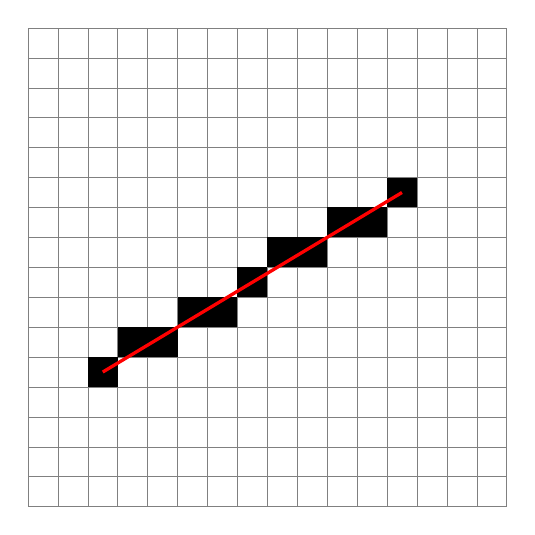
\begin{tikzpicture}
    [
        scale=0.38,
    ]
    
    \foreach \i in {0,...,16} {
        \draw [very thin, gray] (\i, 0) -- (\i, 16);
    }
    \foreach \i in {0,...,16} {
        \draw [very thin, gray] (0, \i) -- (16, \i);
    }
    
    \foreach \x/\y in
    {2/4, 3/5, 4/5, 5/6, 6/6, 7/7, 8/8, 9/8, 10/9, 11/9, 12/10}
    {
        \fill [black] (\x, \y) rectangle (\x + 1, \y + 1);
    }
    \draw [very thick, red] (2.5, 4.5) -- (12.5, 10.5);
    
    \end{tikzpicture}
    \label{fig:pixels}
    \caption{Individual pixels of a line segment}
    \end{figure}
    
    \vfill\columnbreak
    
    \noindent
    If we zoom in on a line displayed on a computer screen (as shown in fig.
    \ref{fig:pixels}), we can see the individual pixels that make up the line.
    Each pixel is an approximation of the line drawn. 
    \vfill
    
\end{multicols}

\subsection{Theory}
A straight line be can described in math by $y = \alpha x + \beta$, where
$\alpha$ is the slope of the line, and $\beta$ is where the line intersects
with the $y$-axis. This equation, however, does not yield a finite line,
therefore we turn to the definition of a straight line, containing the start-
and end-points of the line ${(x,y) | (a,b) \cdot (x - x_0, y - y_0) = 0}$,
by which we describe a straight line as a dot-product of the line vector
$(x - x_0, y - y_0)$ and its normal vector $(a,b)$, which are orthogonal to
each other, making the dot-product zero as a consequence of its geometric
definition $a \cdot b = \norm{a} \norm{b} \cos \theta$, for which the angle
$\theta$ would be $90^{\circ}$ making $\cos \theta = 0$.

Expanding on the above equation, we can derive the homogeneous equation of a
straight line.
\begin{align}
    (a,b) \cdot (x - x_0, y - y_0) &= 0 \\
    a(x - x_0) + b(y - y_0) &= 0 \\
    ax - ax_0 + by - by_0 &= 0 \\
    ax + by \underbrace{- ax_0 - by_0}_{c} &= 0
\end{align}

For later convenience we allow for the contraction $c$. By the above
derivation we have that a line $l$ can be defined by the homogeneous equation.
\begin{align}
    l: \quad {(x,y) | ax + by + c = 0}
\end{align}

Now that we have established a mathematical definition of a straight line, we
can turn our attention toward the problem of approximating a given line
described by these equations. For this purpose we will be using the formula
for the distance from a point to a line.
% prove if time allows it
\begin{align}
    d(x,y) = \frac{(a,b)}{\sqrt{a^2 + b^2}} \cdot (x - x_0, y - y_0)
\end{align}

With this equation we can tell how far away a point may be from the line in
question, moreover it tells us on which side of the line $l$ a point $p$
resides. That is,
\begin{align}
    \text{Point $p$ resides on}
    \begin{cases}
        \text{north of line $l$} &\mbox{iff. $d(x,y) > 0$} \\
        \text{on line $l$} &\mbox{iff. $d(x,y) = 0$} \\
        \text{south of line $l$} &\mbox{iff. $d(x,y) < 0$}
    \end{cases}
    \label{eqn:distance-properties}
\end{align}

By the same expansion as before, we can derive another form of this equation.
\begin{align}
    d(x,y)
    &= \frac{(a,b)}{\sqrt{a^2 + b^2}} \cdot (x - x_0, y - y_0) \\
    &= \frac{a(x - x_0) + b(y - y_0)}{\sqrt{a^2 + b^2}} \\
    &= \frac{ax + by - ax_0 - by_0)}{\sqrt{a^2 + b^2}} \\
    &= \frac{ax + by + c)}{\sqrt{a^2 + b^2}} \\
\end{align}

Now that we have a way of expressing the distance from an arbitrary point
perpendicular to the line, as derived above, we can use this to determine
which pixels lies closest to the line. This in effect allows us to perform the
approximation necessary to produce a rasterization of a straight line.

Before doing so, we would like to reduce unnecessary overhead. Squareroots
are very CPU intensive operations, and so by recognizing that
$\sqrt{a^2 + b^2} > 0$, we can substitute it by multiplying by it, effectively
removing it from the equation. We declare a new function $F(x,y)$ for this
purpose.
\begin{align}
    F(x,y)
    = \frac{ax + by + c}{\sqrt{a^2 + b^2}} \sqrt{a^2 + b^2}
    = ax + by + c
\end{align}

The reason we can expect the properties to be preserved is that we ensured
that since the previous denominator $\sqrt{a^2 + b^2}$ was ensured to be
positive at all times, removing it does not affect the sign, as it was purely
determined by the numerator $ax + by + c$. This proves that the properties
given in (\ref{eqn:distance-properties}) holds for $F(x,y)$ as well.

Under considerations of simplification and maintaining simplicity of the
algorithm itself, assume that $\lvert\frac{\Delta y}{\Delta x}\rvert \leq 1$.
That is, the slope of line $\alpha$ can only take on values in the interval
$[-1;1]$ --- should it exceed, then $\lvert\frac{\Delta x}{\Delta y}\rvert
\leq 1$, which we will use to our advantage in constructing the algorithm. 

Lastly, we need to state that one can substitute the normal vector $(a,b)$ by
$(\Delta y, -\Delta x)$. This can be derived from the linear function $y =
\alpha x + \beta$, which can be rewritten as $x \Delta y - y \Delta x + \beta
\Delta x = 0$.

With all of these derivations of equations and their properties stated, we may
proceed and construct the algorithm.

\section{The Solution}
\subsection{Choosing a point}
Let $p_i$ be the $i$th point with coordinates $(x_i, y_i)$. Under the
assumption that point $p_i$ has been drawn, let $d_p = F(x_i + 1, y_i +
\frac{1}{2}$ be a decision variable that we know the value of. Then by the
assumption that $\alpha \in [-1;1]$ we must decide from the known point $p_i$
whether or not $p_{i + 1}$ lies above or below the line. From the properties
given in (\ref{eqn:distance-properties}) we have that
\begin{align}
    (x_{i + 1}, y_{i + 1}) &=
    \begin{cases}
        (x_i + 1, y_i + 1) &\mbox{iff. $d_p \geq 0$} \\
        (x_i + 1, y_i) &\mbox{iff. $d_p < 0$}
    \end{cases}
\end{align} 

\subsection{The decision variable}
Choosing either we must update the decision variable correspondingly for
$d_{p + 1}$. In the case of $d_p \geq 0$ (above the line), we have that
\begin{align}
    d_{i + 1}
    &= F(x_i + 2, y_i + \frac{3}{2}) \\
    &= a(x_i + 2) + b(y_i + \frac{3}{2}) + c \\
    &= \underbrace{a(x_i + 1) + b(y_i + \frac{1}{2}) + c}_{d_p}
     + \underbrace{a + b}_{\Delta d}
\end{align}
That is, the difference $\Delta d = d_{p + 1} - d_p$ is simply $a + b$.
Correspondingly, if $d_p < 0$ (below the line), we have that
\begin{align}
    d_{i + 1}
    &= F(x_i + 2, y_i + \frac{1}{2}) \\
    &= a(x_i + 2) + b(y_i + \frac{1}{2}) + c \\
    &= \underbrace{a(x_i + 1) + b(y_i + \frac{1}{2}) + c}_{d_p}
     + \underbrace{a}_{\Delta d}
\end{align}
In the same way as before $\Delta d$ is in this case simply $a$.

\subsection{Initializing the algorithm}
Now that we have a way of deciding how to choose a point $p$ and update the
decision variable $d_p$ correspondingly, we can provide the initial values for
these.

We remark that we have at least two definite points beknownst to us; a
starting- and ending point. For the initialization of the point $p_0$, we
simply choose the starting point. Doing so, we can calculate the initial value
of $d_p$.
\begin{align}
    d_0
    &= F(x_0 + 1, y_0 + \frac{1}{2}) \\
    &= a(x_0 + 1) + b(y_0 + \frac{1}{2}) + c \\
    &= \underbrace{ax_0 + by_0 + c}_{0}
     + \underbrace{a + \frac{1}{2}b}_{\Delta d_0}
\end{align}
Under the premise that a point $p \in \mathbb{Z}^2$, then by multiplying each
constituent just discussed --- $d_p$ and $\Delta d_p$ --- by 2 we ensure that
all values calculated are integers, which yields better performance.

We now have all that we need to perform the initialization of the algorithm,
let us briefly list them, for convience and later reference.
\begin{enumerate}
    \item $\Delta x = x_n - x_0$ and $\Delta y = y_n - y_0$
    \item $d = 2 \Delta y - \Delta x$
    \item $\Delta d =
        \begin{cases}
            2(\Delta y + \Delta x) &\mbox{iff. $d \geq 0$} \\
            2 \Delta y &\mbox{iff. $d < 0$}
        \end{cases}$ \\
    \item $step_x =
        \begin{cases}
             1 &\mbox{iff. $\Delta x \geq 0$} \\
            -1 &\mbox{iff. $\Delta x < 0$}
        \end{cases}$ and $step_y =
        \begin{cases}
             1 &\mbox{iff. $\Delta y \geq 0$} \\
            -1 &\mbox{iff. $\Delta y < 0$}
        \end{cases}$ \\
\end{enumerate}
All of which are set on lines 1--11 in the code excerpt (see
\ref{fig:code-excerpt} on page ~\ref{fig:code-excerpt}).

\subsection{Direction Issue}
While we would like to simply draw on either side of the line based upon
whether or not $d \geq 0$, we would also like the algorithm to produce
reliable results. Following this naive approach can yield different results
depending on the direction of the line. That is, when $d = 0$ for a given
point, when $step_x = 1$ the algorithm would choose the pixel above, while
choosing the pixel below if $step_x = -1$. Although the lines should have been
the exact same rendition, interchanging the starting- and ending points of a
line yields different rasterized results, and so this must be accounted for.

A straight-forward solution is to simply check in which direction we are
following the line whenever $d = 0$, and if we are going in the positive
direction, that is $step_x = 1$, then we would want to choose the pixel above,
if not, we stay on the $x$-axis. In the solution code excerpt provided this is
evident on lines $16$ and $30$, on which we declare the check variable, and
are used on lines $20$ and $35$.

\newpage
\subsection{Algorithm}
We present an excerpt from the code, as provided (see the {\tt /src}
directory), containing the algorithm discussed.
\begin{figure}[H]
    \lstinputlisting{figures/algorithm.cpp}
    \label{fig:code-excerpt}
    \caption{Except code containing the actual algorithm}
\end{figure}
The excerpt can be found in the code provided under
{\tt /src/Primitives/Line.cpp}. I will remark that the type {\tt Point2D} is
declared in {\tt /src/Types.h}.

\newpage
\subsection{Tests}
I let my program generate an interesting example, highlighting the direction
issue, and showing that its solution works as expected.
\begin{multicols}{2}

    \begin{figure}[H]
        \center
        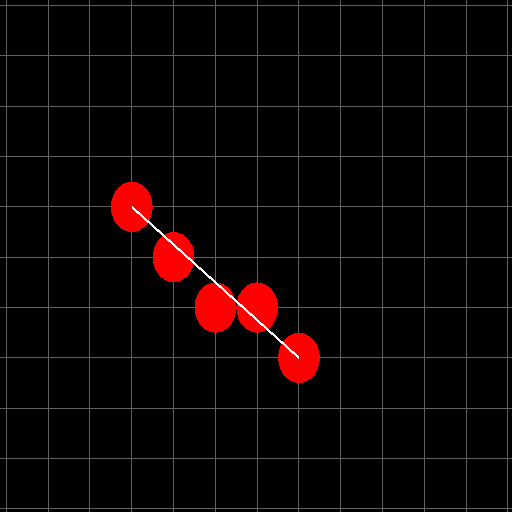
\includegraphics[scale=0.40]{figures/test1.png}
        \caption{Test showing an $x$-dominant left-to-right solution}
    \end{figure}
    \vfill\columnbreak\noindent
    In the example to the left the coords are $(-4, -1)$ to $(0, -4)$, which
    gives us that $\Delta x = 4$ and $\Delta y = 3$, making $x$ the dominant
    axis. And since $\Delta x \geq 0$, then $step_x = 1$, making the algorithm
    go from left to right, which for $x = -2$ hits the case of $d = 0$, and
    since we have established that it is indeed going left to right, we should
    follow $step_y$, which it indeed does.
    \vfill

\end{multicols}

I have deliberately organized my code in such a way, that it is easy to
generate a random line within certain constraints on the coordinates, such
that if need be, then one need not write any code to verify the correctness of
the algorithm, but simply run the program. Hitting the ENTER key will generate
a new random line whilst displaying the starting- and ending points of the
line in the standard output console. Hitting the ESCAPE key quits the program
gracefully.

\end{document}

